% Licensed to the Apache Software Foundation (ASF) under one or more
% contributor license agreements. See the NOTICE file distributed with
% this work for additional information regarding copyright ownership.
% The ASF licenses this file to You under the Apache License, Version 2.0
% (the ``License''); you may not use this file except in compliance with
% the License. You may obtain a copy of the License at
%
% http://www.apache.org/licenses/LICENSE-2.0
%
% Unless required by applicable law or agreed to in writing, software
% distributed under the License is distributed on an ``AS IS'' BASIS,
% WITHOUT WARRANTIES OR CONDITIONS OF ANY KIND, either express or implied.
% See the License for the specific language governing permissions and
% limitations under the License.

\subsubsection{Configuring a Sharepoint Connector}

You must fill in the following tabs if you are configuring a
Sharepoint Connector:

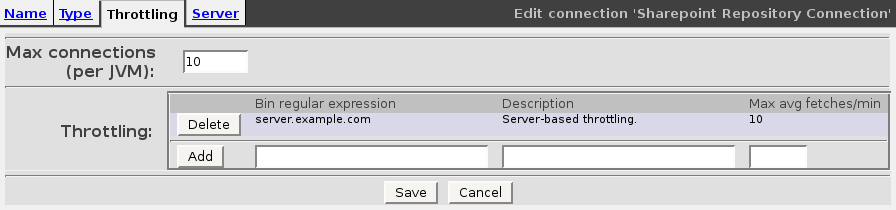
\includegraphics[width=300pt]{shp-edit-repository-tab3}

\begin{itemize}

\item \textbf{Max connections (per JVM):} Here you can set the maximum
number of connections to your repository.  \ifCombinedConnectorGuide
The maximum number of connections per JVM is important for three
reasons; licensing, appliance resources, and the possiblity of
overwhelming the ingestion interface. For a more complete explanation,
see the Max Connections item on page \pageref{maxrepocon}.\fi

\ifJDBCGuide
The maximum number of connections per JVM is important for several
reasons.  First, the number of connections may impact the resources
available on your Sharepoint server.

Second, the number of connections may impact the resources
available on the appliance. If the connector framework is slowing down
your appliance, lowering this number should help.

Third, only ten document streams can be processed by the appliance
at one time.  If you are also using other repository connectors or
the \command{ingest} command on the appliance, you should reduce this
number to prevent contention for the Ingestion interface. The Sharepoint
Connector will never overwhelm the interface on its own, but when other
applications are also using the ingestion interface, it may be best to
set the number of repository connections to five or even fewer.
\fi


\item \textbf{Throttling:} Here you can set a maximum document fetch
rate for the repository connection.  The maximum fetch rate allows you
to set three things: Expression, description, and fetches per minute.

In the Sharepoint Connector, the expression field can be used to
create throttle groups based on server name. Put the server's fully
qualified domain name in the expression field, and set the maximum
average number of document fetches per minute. Once you have set that,
click Add. Creating a throttling group with a blank expression will
throttle all servers together.

\end{itemize}

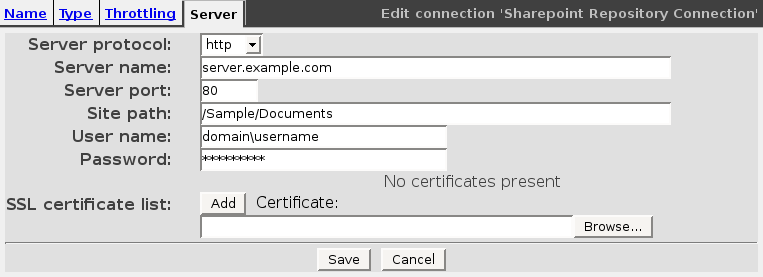
\includegraphics[width=300pt]{shp-edit-repository-tab4}

To fill out this tab, you will need information about the Sharepoint
server with which you wish to connect. One method of determining
protocol, name, and site path information is to browse to the
Sharepoint root or managed site that you wish to crawl, and decompose
the URL into the necessary information. For example, if your
Sharepoint site URL is
\url{http://server.example.com/Sample/Documents/default.aspx}, the
appropriate protocol is \texttt{http}, the server name is
\texttt{server.example.com}, and the site path is
\texttt{/Sample/Documents}. The site path should not include subsite information; subsite information is included during crawler job creation. You may need
to ask your Sharepoint administrator to provide other information.

\begin{itemize}

\item \textbf{Server protocol:} Select ``http'' or ``https'' using the drop down box. The protocol appears at the beginning of the Sharepoint site URL.

\item \textbf{Server name:} The name of your Sharepoint server.

\item \textbf{Server port:} The port to use to connect to the server. You should ask your Sharepoint administrator for the correct port.

\item \textbf{Site path:} The site path for the Sharepoint site on your server that you wish to crawl. This may be blank if you are crawling the root site of your server.

\item \textbf{User name:} This should be the Active Domain user name used by your MetaCarta appliance, in the format \texttt{domain$\backslash$username}.

\item \textbf{Password:} The password corresponding to the user name given.

\item \textbf{SSL certificate list:}
If you specified ``https'' as the server protocol above, you may need to
upload appropriate SSL certificates or certificate authorities here. The
repository connection will need certificates similar to those used to
connect to your Sharepoint site using an Internet browser.

If the certificate authority used to sign your server certificate is a
well-known authority, you will not need to upload a certificate
here. The appliance will automatically accept a certificate from the
server. If the server certificate is signed by an unknown authority,
you should upload the authority's certificate. In some cases, the
authority may be unavailable. In this case, you can upload the
server-side certificate itself. Server-side certificate changes may
require you to upload newer versions of this certificate if you use
this option.

\end{itemize}

\note{If the server you specify on this tab is running Sharepoint Services 3.0 you must install the MetaCarta Sharepoint Web Service on that server. See page \pageref{SWService} for instructions on installing the Sharepoint Web Service.}


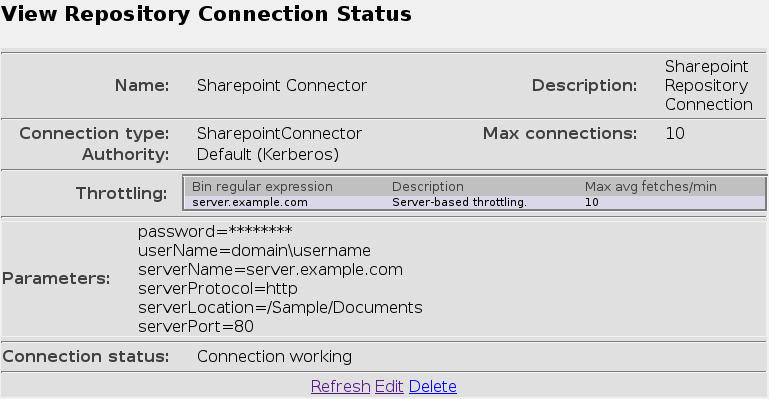
\includegraphics[width=300pt]{shp-view-repo-conn-status}

In this example (which does not contain accurate information for any
Sharepoint Connector), the Connection Status is ``Connection
working.'' If connetion has failed, the status message may contain
information about the failure.  If you see an error message, you most
likely have incorrectly entered one of the fields, and should click
``Edit'' to fix the data. If you have entered everything as you
intended, please inform your database administrator; you may not have
been given the correct information.
